\chapter{Statistics of the overlap distribution}
\label{chap:overlap}

\section{Introduction}

Despite much debate, there is still no consensus on the nature of the
spin-glass state. According to the ``replica symmetry breaking" (RSB) picture
of Parisi discussed in \cref{sec:intro-rsb}, there are many ``pure states," a
nontrivial order parameter distribution, and a line of transitions in a
magnetic field, the de Almeida-Thouless (AT) line. By contrast, according to
the droplet theory, there is only a symmetry-related pair of pure states in
zero field (one state in a nonzero field), and thus the order parameter
distribution is trivial in the thermodynamic limit and there is no AT line. The
nature of the spin glass phase has been investigated in a series of papers by
Newman and Stein (see, for example, \textcite{stein2013spin} and references
therein), and recently by \textcite{read2014short}.
\textcite{marinari2000replica} discuss the RSB point of view.
% TODO: clarify last sentence

The sample-averaged order parameter distribution, defined in
\cref{eq:sample-pofq,eq:pofq} below, is predicted to be nonzero in the vicinity
of $q=0$ as the size of the system $N \equiv L^d$ tends to infinity, according
to the RSB picture \autocite{parisi1983order}, whereas it is expected to
\emph{vanish} as $L^{-\theta}$ in the droplet picture, where $\theta$ is a
positive ``stiffness" exponent \autocite{fisher1986ordered}.
% TODO: ref discussion in intro
Results from simulations%
\footnote{%
  \textcite{%
    marinari2000replica,%
    reger1990monte,%
    katzgraber2001monte,%
    katzgraber2003monte%
  }
}
seem close to the predictions of RSB, but it has been argued
\autocite{moore1998evidence,middleton2013extracting} that the sizes which can
be simulated are too small to see the asymptotic behavior.

Consequently, there has recently been interest%
\footnote{%
  \textcite{%
    middleton2013extracting,%
    yucesoy2012evidence,%
    monthus2013typical%
  }
}
in studying other quantities related to $P(q)$ but where more attention is paid
to the overlap distribution of \emph{individual} samples, $\sample{P}(q)$,
rather than just the sample average. Accurately determining $\sample{P}(q)$ for
each sample is more demanding numerically than just computing the average,
% TODO: explain why
but computer power has advanced to the point where this is now feasible.

Here we will study in detail these new quantities for a \emph{range} of models.
In addition to the short-range Edwards-Anderson (EA) spin-glass models in three
and four space dimensions, and the infinite-range Sherrington-Kirkpatrick (SK)
model, we also study diluted long-range (LR) Ising spin-glass models in one
space dimension, described in detail in \cref{sec:nonextensive-motivation}. The
LR models are are useful here because it is important to study models in the
mean-field regime ($d \geq 6$), or equivalently $\sigma < 2/3$, but it is
difficult to simulate and carry out a finite-size scaling (FSS) analysis of the
results for short-range models in high dimensions because the number of spins
grows so quickly with $L$ that only a few sizes can be considered. The LR
models do not have this difficulty, so we use them to probe the mean-field
regime. Finally, verifying the consistency of our results for the SR and LR
models gives us additional confidence in our numerical results.


\section{Models}
\label{sec:overlap-models}

We study several classes of Ising spin-glass models. These are one-dimensional
long-range (LR) models, three- and four-dimensional short-range (EA) models,
and the infinite-range (SK) model. In all cases the Hamiltonian can be written
in the form
\begin{equation}
  \ham = -\sum_{i,j} J_{ij} S_i S_j,
\end{equation}
where the $S_i \in \cbr{1,2,\dots,N}$ represent Ising spins that take values
$\pm 1$, and the $J_{ij}$ are independent, quenched
% TODO: explain "quenched"
random variables. The summation is defined over all pairs of interacting spins.
All of the models studied here have finite-temperature spin-glass transitions.
The models differ according to which spins interact and the strength of the
couplings.


\subsection{Edwards-Anderson models on hypercubic lattices}

The three- and four-dimensional EA models that we study are defined on
(hyper-)cubic lattices with periodic boundary conditions. The nearest-neighbor
interactions are taken from a Gaussian distribution with zero mean and unit
variance,
\begin{equation}
  \dav{J_{ij}}=0,\quad
  \dav{J_{ij}^2}=1,
\end{equation}
where $\dav{\dots}$ indicates a quenched average over the couplings.
% TODO: "quenched average"?
From numerical studies it is known that the transition temperatures are
$T_c=0.951(9)$ for $d=3$ \autocite{katzgraber2006universality}
and $T_c=1.80(1)$ for $d=4$ \autocite{parisi1996equilibrium}.


\subsection{Sherrington-Kirkpatrick model}

In the SK model each spin interacts with every other spin. The couplings
are taken from a Gaussian distribution with zero mean and variance which
is inversely proportional to the size of the system,
\begin{equation}
  \dav{J_{ij}}=0,\quad
  \dav{J_{ij}^2}=1/N.
\end{equation}
The latter condition is necessary to ensure that there is a well-defined
thermodynamic limit, as discussed in \cref{sec:nonextensive-motivation}. The
transition temperature for this model is $T_c=1$
\autocite{sherrington1975solvable}.


\subsection{One-dimensional diluted long-range model}

For the LR models the distribution of the interactions satisfies
\begin{equation}
  \dav{J_{ij}} = 0,\quad
  \dav{J_{ij}^2} \propto R_{ij}^{-2\sigma},
  \label{eq:J-mean-var-lr-3}
\end{equation}
where $\sigma$ is a parameter controlling the range of interactions, and
$R_{ij}$ is the chord distance between sites $i$ and $j$ when the spins are
arranged on a ring, see \cref{fig:1dlr-chord,eq:chord-distance}. The
\emph{diluted model} corresponds to a choice of the distribution $P(J_{ij})$
which satisfies \cref{eq:J-mean-var-lr-3} while allowing for efficient computer
simulation, namely
\begin{equation}
  P(J_{ij})
  = (1-p_{ij})\delta(J_{ij}) + p_{ij}\frac{1}{\sqrt{2\pi}} e^{-J_{ij}^2/2},
\end{equation}
where $p_{ij} \propto R_{ij}^{-2\sigma}$ at large distance. The constant of
proportionality is determined by fixing the mean number of neighbors of each
spin, $z_b$. In this work we take $z_b=6$. The motivation for choosing this
distribution and the algorithm used to sample from it are discussed in
\cref{sec:nonextensive-models}.

We consider three values of the range parameter: $\sigma=0.6$, which is in the
mean-field regime \autocite{larson2010numerical}, $\sigma=0.784$, which
represents, at least approximately, a short-range system in four dimensions,%
\footnote{%
  \label{note:equiv}
  \textcite{%
    larson2010numerical,%
    banos2012correspondence,%
    katzgraber2009ultrametricity,%
    larson2013spin%
  }
}
and $\sigma=0.896$, which approximately represents a three-dimensional system.%
\footnote{See \cref{note:equiv}.}
The values of $T_c$ are approximately equal to 1.35 and 0.795 for $\sigma=0.784$
and 0.896, respectively \autocite{larson2013spin}. For $\sigma=0.6$ we find
$T_c \approx 1.953$.
% TODO: compare/ref value in dynamics chapter


\section{Methods}

We have carried out parallel-tempering (replica-exchange) Monte Carlo
simulations of the models described in \cref{sec:overlap-models}. In parallel
tempering, $N_T$ replicas of the system with the same couplings are each
simulated at a different temperature in the range between $T_{\mathrm{min}}$
and $T_{\mathrm{max}}$. In addition to standard Metropolis sweeps at each
temperature, there are parallel tempering moves that allow replicas to be
exchanged between neighboring temperatures. Parallel tempering moves permit
replicas to diffuse from low temperatures, where equilibration is very slow, to
high temperatures, where it is easy, and back again. The result is greatly
accelerated equilibration relative to an algorithm that only performs
Metropolis sweeps. See \cref{sec:numerical-parallel-tempering} for more on the
theory and implementation the parallel tempering algorithm.

The simulation parameters are given in
\cref{%
  tab:overlap-params-1dlr,%
  tab:overlap-params-3d,%
  tab:overlap-params-4d,%
  tab:overlap-params-sk%
}.
A single ``sweep" consists of a Metropolis sweep at each temperature, followed
by parallel tempering moves between each pair of neighboring temperatures. The
parameter $b$ determines the number of sweeps: $2^b$ for equilibration followed
by $2^b$ for data collection. The parameter $N_{\mathrm{sa}}$ is the number of
disorder samples simulated.
For each model we have chosen the lowest temperature to be less than or equal
to $0.4 T_c$, the approximate temperature for which we report most of our results.

\pgfplotstableset{params/.style={
    /pgf/number format/set thousands separator={},
    columns/sigma/.style={
      column name={$\sigma$},
      dec sep align,
      precision=3},
    columns/N/.style={
      column type={r},
      column name={$N$}},
    columns/L/.style={
      column type={r},
      column name={$L$}},
    columns/Tmin/.style={
      column name={$T_{\mathrm{min}}$},
      dec sep align,
      precision=4
    },
    columns/Tmax/.style={
      column name={$T_{\mathrm{max}}$},
      dec sep align,
      precision=4
    },
    columns/b/.style={column name={$b$}},
    columns/NT/.style={column name={$N_T$}},
    columns/Nsa/.style={column name={$N_{\mathrm{sa}}$}},
  }}

\begin{table}
  \centering
  \pgfplotstabletypeset[params]{data/overlap-params-1dlr.csv}
  \caption [
    Simulation parameters for one-dimensional long-range spin-glass models with
    diluted bonds.
  ]
  {
    Simulation parameters for the 1D LR models. For each value of $\sigma$ and
    size $N$, $N_{\mathrm{sa}}$ samples were equilibrated for $2^b$ sweeps and
    then measured for an additional $2^b$ sweeps, using replica-exchange Monte
    Carlo with $N_T$ temperatures between $T_{\mathrm{min}}$ and
    $T_{\mathrm{max}}$.
  } \label{tab:overlap-params-1dlr}
\end{table}

\begin{table}
  \centering
  \pgfplotstabletypeset[params]{data/overlap-params-3d.csv}
  \caption[
    Simulation parameters for the three-dimensional Edwards-Anderson spin glass.
  ]
  {
    Simulation parameters for the 3D EA spin glass. The parameters are defined
    as in \cref{tab:overlap-params-1dlr} except for the linear size $L$, where
    $N=L^3$.
  }
  \label{tab:overlap-params-3d}
\end{table}

\begin{table}
  \centering
  \pgfplotstabletypeset[params]{data/overlap-params-4d.csv}
  \caption[
    Simulation parameters for the four-dimensional Edwards-Anderson spin glass.
  ]
  {
    Simulation parameters for the 4D EA spin glass. The parameters are defined
    as in \cref{tab:overlap-params-1dlr} except for the linear size $L$, where
    $N=L^4$.
  }
  \label{tab:overlap-params-4d}
\end{table}

\begin{table}
  \centering
  \pgfplotstabletypeset[params]{data/overlap-params-sk.csv}
  \caption[
    Simulation parameters for the Sherrington-Kirkpatrick spin glass.
  ]
  {
    Simulation parameters for the SK spin glass. The parameters are defined as
    in \cref{tab:overlap-params-1dlr}.
  }
  \label{tab:overlap-params-sk}
\end{table}

To test our simulations for equilibration, we use the method discussed in
\cref{sec:equilibration-test-gaussian}. That is, we plot \cref{eq:delta} as a
function of the number of sweeps and infer the time to reach equilibrium from
when $\Delta(t)$ is consistent with zero for a sufficient number of points, see
the discussion below. Note that for the SK model, $\tcmfsq=T_c^2=1$, while for
the remaining models $\tcmfsq=z$, where $z$ is the (average) number of
neighbors of each site. Thus $z=2d$ for the EA models and $z=z_b=6$ for the LR
models.

While the method of \cref{sec:equilibration-test-gaussian} is a useful
criterion for the equilibration of \emph{sample-averaged} quantities, we must
be especially careful when studying quantities that may be sensitive to the
equilibration of individual samples, such as those considered in
\cref{sec:overlap-quantities}. To ensure the equilibration of individual
samples, \emph{i.e.} not just sample averages, we run our simulations for many
times the number of sweeps needed to satisfy \cref{eq:delta}; at minimum we
require that at least 3 consecutive, logarithmically-spaced times agree within
error bars.

\Cref{fig:overlap-equil} shows example equilibration tests for
\subref{fig:overlap-equil-1dlr} the 1D LR model with $\sigma=0.896$ for the
largest size at the lowest temperature, and \subref{fig:overlap-equil-3d} the
3D EA model with $L=8$, again at the lowest temperature. In both cases the data
plateau at zero (within the error bars) at around $10^5$ sweeps, but the
simulations continue for much longer than this to ensure that individual
samples are equilibrated.

\begin{figure}
  \centering
  \begin{subfigure}{0.49\textwidth}
    \centering
    \includestandalone{figures/delta_eq-1dlr}
    \subcaption{1D LR model}
    \label{fig:overlap-equil-1dlr}
  \end{subfigure}
  \begin{subfigure}{0.49\textwidth}
    \centering
    \includestandalone{figures/delta_eq-3d}
    \subcaption{3D EA model}
    \label{fig:overlap-equil-3d}
  \end{subfigure}
  \caption[
    Example equilibration plots for the three-dimensional Edwards-Anderson
    model and the one-dimensional long-range model.
  ]
  {
    Plots of the quantity $\Delta(t)$, defined in \cref{eq:delta}, for
    \subref{fig:overlap-equil-3d} the 3D EA model and
    \subref{fig:overlap-equil-1dlr} the 1D LR model. The results shown are for
    the lowest temperatures studied and intermediate sizes. Note that at large
    times $\Delta \to 0$, indicating the equilibration of \emph{sample
      averages}, but the simulations continue well beyond this point to ensure
    that individual samples are equilibrated. Error bars are smaller than the
    symbols.
  }
  \label{fig:overlap-equil}
\end{figure}

As an additional check of equilibration for the 1D LR models,
\cref{fig:overlap-stats-vs-time} shows several quantities of interest, defined
in \cref{sec:overlap-quantities}, as a function of the number of sweeps on a
log scale, for the lowest temperature studied and for each value of $\sigma$.
The data appear to have saturated. The 3D EA data have also been tested for
equilibration using the integrated autocorrelation time, as discussed in
\textcite{yucesoy2013correlations}.

\begin{figure}
  \centering
  \begin{subfigure}[b]{0.32\textwidth}
    \centering
    \includestandalone{figures/delta-vs-t-1dlr}
    \subcaption{$\Delta(q_0=0.2,\,\kappa=1)$}
    \label{fig:delta-vs-t-1dlr}
  \end{subfigure}
  \begin{subfigure}[b]{0.32\textwidth}
    \centering
    \includestandalone{figures/Iav-vs-t-1dlr}
    \subcaption{$I^{\mathrm{av}}(q=0.2)$}
    \label{fig:Iav-vs-t-1dlr}
  \end{subfigure}
  \begin{subfigure}[b]{0.32\textwidth}
    \centering
    \includestandalone{figures/Imed-vs-t-1dlr}
    \subcaption{$I^{\mathrm{med}}(q=0.2)$}
    \label{fig:Imed-vs-t-1dlr}
  \end{subfigure}
  \caption[
    Plots of various statistics of the spin overlap distribution as a function
    of Monte Carlo time, indicating that the quantities have reached a steady
    state.
  ]
  {
    Plots of several observables obtained from the overlap distribution,
    defined in \cref{sec:overlap-quantities}, versus the number of Monte Carlo
    sweeps for the largest size studied, $N=1024$, for the long-range model at
    the lowest temperature simulated for each value of $\sigma$. (See
    \cref{tab:overlap-params-1dlr}.) The data appear to have reached a steady
    state.
  }
  \label{fig:overlap-stats-vs-time}
\end{figure}


\section{Measured quantities}
\label{sec:overlap-quantities}

For a single sample $\mathcal{J}\equiv\cbr{J_{ij}}$, the spin overlap
distribution is given by

\begin{equation}
  \sample{P}(q) = \av{\delta\del{q - \frac{1}{N}\sum_{i=1}^N S_i^{(1)} S_i^{(2)}}},
  \label{eq:sample-pofq}
\end{equation}
where ``(1)" and ``(2)" refer to two independent copies of the system with the
same interactions, and $\av{\cdots}$ denotes a thermal (\emph{i.e.} Monte
Carlo) average for a single sample. In most previous work, $\sample{P}(q)$
is simply averaged over disorder samples to obtain $P(q)$ defined by
\begin{equation}
  P(q) = \dav{\sample{P}(q)}
  \label{eq:pofq}
\end{equation}

In order to gain additional information that might distinguish the RSB and
droplet pictures, several investigators have recently introduced other
observables related to the statistics of $\sample{P}(q)$.
\textcite{yucesoy2012evidence} proposed a measure that is sensitive to peaks in
the overlap distributions of \emph{individual samples}, $\sample{P}(q)$. A
sample is counted as ``peaked" if $\sample{P}(q)$ exceeds a threshold value
$\kappa$ in the domain $\abs{q} < q_0$. The quantity $\Delta(q_0,\kappa)$ is
then defined as the fraction of peaked samples. More precisely, for each sample
let
\begin{equation}
  \sample{\Delta}(q_0,\kappa) =
  \begin{cases}
    1 & \text{if $\sample{P}(q)>\kappa$ for some $q$ where $\abs{q}<q_0$}, \\
    0 & \text{otherwise.}
  \end{cases}
  \label{eq:delta-sample}
\end{equation}
We then define $\Delta(q_0,\kappa)$ to be the sample average,
\begin{equation}
  \Delta(q_0,\kappa) = \dav{\sample{\Delta}(q_0,\kappa)}.
  \label{eq:delta-average}
\end{equation}
Note that $\Delta(q_0,\kappa)$ is a nondecreasing function of $q_0$ and a
nonincreasing function of $\kappa$. A more important property of
$\Delta(q_0,\kappa)$ is that its behavior for $N \to \infty$ distinguishes
between the RSB and droplet pictures as follows. All of the scenarios for the
low-temperature behavior of spin-glass models predict that $\sample{P}(q)$ is a
superposition of $\delta$ functions as $N \to \infty$. The difference between
scenarios lies in the number and positions of these $\delta$ functions, see
\cref{fig:pq-droplet-rsb}. According to the RSB picture, there is a countable
infinity of $\delta$ functions that densely fill the line between $-\qea$ and
$+\qea$. Thus, for any $q_0$ and any $\kappa$, $\Delta(q_0,\kappa) \to 1$ for
models described by RSB. On the other hand, for models described by the droplet
scenario or other scenarios with only a single pair of pure states for $N \to
\infty$, $\Delta(q_0,\kappa) \to 0$ for any $q_0<\qea$ and any $\kappa$. Thus,
the quantity $\Delta(q_0,\kappa)$ will sharply distinguish the RSB and droplet
scenarios if one can study large enough sizes. We will study the size
dependence of $\Delta$ numerically for all of our models in
\cref{sec:overlap-results-delta}.
\begin{figure}
  \centering
  \begin{subfigure}{0.49\textwidth}
    \centering
    \includestandalone{figures/sample-overlaps-Tmin}
    \subcaption{}\label{fig:sample-overlaps-Tmin}
  \end{subfigure}
  \begin{subfigure}{0.49\textwidth}
    \centering
    \includestandalone{figures/sample-overlap}
    \subcaption{}\label{fig:sample-overlap}
  \end{subfigure}
  \caption
  [
    Plots of the overlap distribution $P_{\JJ}(q)$ for individual disorder
    samples.
  ]
  {
    Plots of the overlap distribution $P_{\JJ}(q)$ for individual disorder
    samples. Panel~\subref{fig:sample-overlaps-Tmin} shows the overlap
    distribution obtained for three different samples for the 1D LR model with
    $\sigma=0.784$ at the lowest temperature simulated, $T=0.55$. According to
    \cref{eq:delta-sample} with parameters $q_0=0.2$, $\kappa=1$ (indicated by
    vertical lines and a horizontal line respectively), two of the three
    samples contribute to $\Delta(q_0,\kappa)$.
    Panel~\subref{fig:sample-overlap} shows the overlap distribution $P(q)$
    versus temperature for a single disorder sample for the same model, showing
    the emergence of multiple pairs of peaks below the transition temperature
    $T_c \approx 1.35$.
  }
\end{figure}

As mentioned above, most previous work evaluated the \emph{average} probability
distribution $P(q)$, but recently
\textcite{middleton2013extracting,monthus2013typical}
have proposed measures yielding a \emph{typical} value of the sample
distribution $\sample{P}(q)$ with the hope that these measures would provide a
clearer differentiation between the RSB and droplet pictures than the average
$P(q)$.

\textcite{middleton2013extracting} studied $I^{\mathrm{med}}(q)$, the
\emph{median} of the \emph{cumulative} overlap distribution of a single sample
$\sample{I}(q)$, where $\sample{I}(q)$ is defined by
\begin{equation}
  \sample{I}(q) = \int_{-q}^q \dif q^{\prime} \sample{P}(q^{\prime}).
\end{equation}
We also denote by $I^{\mathrm{av}}(q)$ the sample-averaged cumulative
distribution, which is given by
\begin{equation}
  I^{\mathrm{av}}(q) = \int_{-q}^q \dif q^{\prime} P(q^{\prime}).
  \label{eq:Iav}
\end{equation}
Compared to the average, the median is insensitive to the effect of samples
with unusually large values of $\sample{I}(q)$.

For the SK model $P(q)$ tends to a constant as $q \to 0$, and so
$I^{\mathrm{av}}(q) \propto q$ for small $q$. We can obtain a rough idea of how
$I^{\mathrm{med}}(q)$ varies with $q$ for small $q$ in the SK model from the
results of \textcite{mezard1984nature}. First of all, to obtain a notation
which is more compact and is extensively used in other work, we write $x(q)
\equiv I^{\mathrm{av}}(q)$. \textcite{mezard1984nature} argue that, at small
$q$ where $x(q)$ is also small, the probability of a certain integrated value
$\sample{I}$ is given by
\begin{equation}
  p(\sample{I}) \propto x \sample{I}^{x-1}.
  \label{eq:pofI}
\end{equation}
From \cref{eq:pofI} we estimate the median in terms of the average as
\begin{equation}
  I^{\mathrm{med}}(q) \propto e^{-\ln 2 / x(q)} = e^{-\ln 2/\sbr{2 q P(0)}}
  \label{eq:median-small-q}
\end{equation}
for $q \to 0$, where we used that $P(0)$ is nonzero so $x(q) \equiv
I^{\mathrm{av}}(q) \simeq 2 P(0) q$ in this limit [see \cref{eq:Iav}].
Therefore the median tends to zero exponentially fast as $q \to 0$, whereas the
average only goes to zero linearly.

In the droplet picture, $P(0)$ is expected to vanish with $L$ as $L^{-\theta}$,
so $I^{\mathrm{av}}(q) \propto L^{-\theta} q$ for small $q$.
The median value $I^{\mathrm{med}}(q)$ will presumably also vanish for small $q$
as $L \to \infty$, but we are not aware of any precise predictions for this.
We will study the median cumulative distribution numerically in
\cref{sec:overlap-results-cumulative}.

Another measure related to the overlap distribution of individual samples has
been proposed by \textcite{monthus2013typical}. They suggest calculating a
``typical" overlap distribution defined by the exponential of the average of
the log, \emph{i.e.}
\begin{equation}
  P^{\mathrm{typ}}(q) = \exp\dav{\ln\sample{P}(q)}.
  \label{eq:pofq-typical}
\end{equation}
We will study this quantity numerically in \cref{sec:overlap-results-typical}.

% TODO: density?


\section{Results}

\subsection{Fraction of peaked samples, $\Delta(q_0,\kappa)$}
\label{sec:overlap-results-delta}

Plots of $\Delta(q_0,\kappa)$ for the 1D LR models for various values of $q_0$
and $\kappa$ are given in \cref{fig:delta-1dlr}; corresponding plots for the 3D
and 4D EA models are shown in \cref{fig:delta-ea}. A comparison with the SK
model is made in both cases. The error bars for all plots in this section are
one standard deviation statistical errors due to the finite number of samples.
There are also errors in the data for each sample due to the finite length of
the data collection. For the EA and SK models, we estimated these errors by
measuring $\Delta^+(q_0,\kappa)$ and $\Delta^-(q_0,\kappa)$, defined as in
\cref{eq:delta-sample,eq:delta-average}, but from the $q>0$ and $q<0$
components of $\sample{P}(q)$, respectively. These are expected to be
reasonably independent and their differences provide an estimate of the error
due to finite run lengths. For all sizes, the average absolute difference
between these quantities,
$\sbr{\abs{\Delta^+(q_0,\kappa)-\Delta(q_0,\kappa)}
     +\abs{\Delta^-(q_0,\kappa)-\Delta(q_0,\kappa)}}/2$,
is less than the statistical error.
\begin{figure}
  \centering
  \includestandalone{figures/delta-1dlr}
  \caption[
    Peak-counting statistic $\Delta(q_0,\kappa)$ for one-dimensional long-range
    spin glasses and the Sherrington-Kirckpatrick model.
  ]
  {
    $\Delta(q_0,\kappa)$ as a function of system size $N$ for the 1D LR
    models and the SK model for all available values of $\sigma$ and various
    values of the window $q_0$ and threshold $\kappa$. In all cases the
    temperature is $0.4 T_c$. All panels have the same horizontal scale, and
    all panels in a row have the same vertical scale.
  }
  \label{fig:delta-1dlr}
\end{figure}

\begin{figure}
  \centering
  \includestandalone{figures/delta-ea}
  \caption[
    Peak-counting statistic $\Delta(q_0,\kappa)$ for the three- and
    four-dimensional Edwards-Anderson models and the Sherrington-Kirkpatrick
    model.
  ]
  {
    $\Delta(q_0,\kappa)$ as a function of system size $N$ for the EA models and
    the SK model for several values of the window $q_0$ and threshold value
    $\kappa$. The temperatures are $0.4 T_c$ for the 3D data and $0.5 T_c$ for
    the 4D data. All panels in a column have the same horizontal scale.
  }
  \label{fig:delta-ea}
\end{figure}

One can draw several qualitative conclusions from these plots. It is apparent
that $\Delta(q_0,\kappa)$ is an increasing function of $N$ for small $N$. As
the system size increases, we expect $\Delta(q_0,\kappa)$ to increase because
all the features of $\sample{P}(q)$ sharpen. For the SK model, which is
described by the RSB picture, the number of features and their height should
both increase and $\Delta(q_0,\kappa)$ should be a strongly increasing function
of $N$. Indeed, this behavior is seen except for $\kappa=0.5$, which is a
sufficiently small value that $\Delta(q_0,\kappa)$ is effectively measuring
whether or not there is a feature in the relevant range, and this quantity
increases relatively slowly for the SK model.

However, as $\sigma$ increases for the 1D LR models, the curves become
increasingly flat and the difference between $\sigma=0.896$ and the SK model is
striking; the former is nearly flat while the latter increases sharply (see
\cref{fig:delta-1dlr}). The same qualitative distinction holds between the 3D
EA model and the SK model (see \cref{fig:delta-ea}). The similarity between the
behavior of the 1D model for $\sigma=0.896$ and the 3D EA model is expected
since the two models are believed to have the same qualitative behavior.
% TODO: briefly explain/ref?
The distinction between the SK model and the 1D LR model with $\sigma=0.784$
and the 4D EA model is less striking but qualitatively similar.

It is interesting to compare the results for the SK model with the 1D LR model
with $\sigma=0.6$, which is in the mean-field regime. For $\kappa=0.5$ the
results for the two models are very similar and do not increase much with $N$,
indicating that $\kappa=0.5$ is too small to give useful information for this
range of sizes, as discussed above. For $\kappa=1$, the SK data increase most
rapidly with $N$, and the $\sigma=0.6$ data increase less quickly, but still
faster than the other values of $\sigma$. For $\kappa=2$, the SK data increase
quickly, while for the value of $\sigma$ furthest from the SK limit, 0.896, the
data are moderately large but roughly size-independent over the range of sizes
studied. Curiously, for intermediate values of $\sigma$ (0.6 and 0.784) the
data are very small but show an increase for the larger sizes. This increase is
particularly sharp for $\sigma=0.6$. It seems that there is an initial value of
$\Delta$ for small $N$ and a growth as $N$ increases. We do not have a good
understanding of the initial value, \emph{e.g.}, why it is so small for
$\kappa=2$ and $\sigma=0.6$, 0.784. The more important aspect of the data is
the increase observed, at least for most parameter values, at large sizes.
Given the rapid increase in the data for $\sigma=0.6$, $\kappa=2$ for the
largest size, we anticipate that for still larger sizes, its value for $\Delta$
for $\kappa=2$ would be closer to that of the SK model than that of the
intermediate $\sigma$ values.

There are two possible interpretations of the trends discussed above. If one
believes that the RSB picture holds for all of the models studied here, then
one can point to the fact that all of the $\Delta$ curves are nondecreasing and
assert that they will all approach unity as $N \to \infty$, just extremely
slowly for the 3D EA model and the 1D LR model with $\sigma=0.896$.
\textcite{billoire2013comment} argue that this is the case, and are rebutted by
\textcite{yucesoy2013yucesoy}. If, on the other hand, one believes that the
droplet scenario or chaotic pairs scenario holds for finite-dimensional spin
glasses, then the flattening of the curves for these models is a prelude to an
eventual decrease to zero. Unfortunately, the sizes currently accessible to
Monte Carlo simulation do not permit one to sharply distinguish between these
competing hypotheses. Using an exact algorithm for the two-dimensional (2D)
Ising spin glass with bimodal disorder, \textcite{middleton2013extracting}
shows that the crossover to decreasing behavior for $\Delta(q_0,\kappa)$ in 2D
does occur at large length scales. He also shows, within a simplified droplet
model, that the large length scales are needed to see the predictions of the
droplet scenario manifest in the 3D EA model. Overall, we see that we need
larger sizes to unambiguously determine from $\Delta(q_0,\kappa)$ whether the
droplet of RSB picture applies to 3D-like models.


\subsection{Median $I^{\mathrm{med}}(q)$ and mean $I^{\mathrm{av}}(q)$
  cumulative overlap distribution}
\label{sec:overlap-results-cumulative}

In this section, we compare the mean $I^{\mathrm{av}}(q)$ and the median
$I^{\mathrm{med}}(q)$ of the cumulative overlap distribution.
\Cref{fig:cumulative-stats-1dlr} shows the results for these two quantities for
the SK model and several 1D LR models for a temperature close to $0.4 T_c$.
\Cref{fig:cumulative-stats-ea} shows the same quantities for the 3D and 4D EA
models.

\begin{figure}
  \centering
  \includestandalone{figures/qcdf-1dlr}
  \caption[
    Mean and median over samples of the cumulative overlap distribution for
    one-dimensional long-range and Sherrington-Kirkpatrick spin-glass models.
  ]
  {
    Mean and median over samples of the cumulative distribution $\sample{I}(q)$
    for the 1D LR models and the SK model. In all cases the temperature is
    close to $0.4 T_c$. For both the SK and the 1D models, the median shows a
    relatively strong size dependence compared with the mean, this difference
    being the least pronounced for $\sigma=0.896$. The ``theory" curve for the
    SK data\ [\cref{eq:median-small-q}] is expected to be valid for small $q$
    only. The theory expression can be mulitplied by an (unknown) constant
    which has been set to unity.
    % TODO: understand
    All panels have the same horizontal and vertical scales. Only a representative
    set of points is shown but the curves go through all the points.

  }
  \label{fig:cumulative-stats-1dlr}
\end{figure}

\begin{figure}
  \centering
  \begin{subfigure}{0.49\textwidth}
    \centering
    \includestandalone{figures/qcdf-3d}
    \subcaption{3D EA}\label{fig:cumulative-stats-3d}
  \end{subfigure}
  \begin{subfigure}{0.49\textwidth}
    \centering
    \includestandalone{figures/qcdf-4d}
    \subcaption{4D EA}\label{fig:cumulative-stats-4d}
  \end{subfigure}
  \caption[
    Mean and median over samples of the cumulative overlap distribution for
    three- and four-dimensional Edwards-Anderson spin-glass models.
  ]
  {
    Log-linear plot of $I^{\mathrm{med}}(q)$ and $I^{\mathrm{av}}(q)$ versus
    $q$ for \subref{fig:cumulative-stats-3d} the 3D EA model at $T \simeq 0.42$
    and \subref{fig:cumulative-stats-4d} the 4D EA model at $T \simeq 0.90$.
  }
  \label{fig:cumulative-stats-ea}
\end{figure}

As noted in earlier work,
% TODO: cite
the results for the average show very little size dependence for all models.
This is a prediction of the RSB picture which certainly applies to the SK
model. By contrast, in the droplet picture $I^{\mathrm{av}}(q)$ is predicted to
vanish as $L^{-\theta}$ \autocite{fisher1986ordered}. The observed independence
of $I^{\mathrm{av}}(q)$ with respect to $L$ is one of the strongest arguments
in favor of the RSB picture for finite-dimensional Ising spin-glass models.
However, it has been argued, \emph{e.g.} by
\textcite{moore1998evidence,middleton2013extracting}, that there are strong
finite-size corrections and that the asymptotic behavior predicted by the
droplet model for $I^{\mathrm{av}}(q)$ would only be seen for sizes larger than
those accessible in simulations. For this reason
\textcite{middleton2013extracting} proposes the median as an alternative to the
mean.

The data for the median of the SK model in \cref{fig:cumulative-stats-1dlr}
show a rapid decrease at small $q$, which is \emph{very strongly
  size-dependent}. As discussed in \cref{sec:overlap-quantities} above, the
rapid decrease is expected in the RSB picture since it predicts that
$I^{\mathrm{med}}(q)$ is exponentially small in $1/q$ [see
\cref{eq:median-small-q}]. The theoretical result is shown as a solid line in
the SK panel. It is plausible that the data will approach the theory in the
large $N$ limit, but there are strong finite-size effects at small $q$ for
sizes that can be simulated, so the data for the largest sizes are still far
from the theoretical prediction. This already indicates that the median is not
a very useful measure to distinguish the RSB picture from the droplet picture.

The median data for the 1D LR model with $\sigma=0.6$, which is in the
mean-field regime, shows similar trends to that for the SK model. On the other
hand, for the long-range model furthest from mean-field theory, $\sigma=0.896$,
the data also decrease rapidly at small $q$ but are less dependent on size. The
data for the 3D and 4D EA models in \cref{fig:cumulative-stats-ea} also show a
rapid decrease at small $q$ which is quite strongly size-dependent.

We have seen that even for the SK model it would be very difficult to
extrapolate the numerical data to an infinite system size. For the 1D LR
models, the most likely candidate for droplet theory behavior, according to
which the median (such as the average) vanishes in the thermodynamic limit, is
$\sigma=0.896$. However, for this model, the data are not zero for small $q$
and there is rather little size dependence, implying that, if the droplet
picture does hold, it will only be seen for much larger sizes than can be
simulated. This is the same situation as for the mean (if the droplet picture
is correct). Consequently, it does not seem to us that the median of the
cumulative order parameter distribution is a particularly useful quantity to
distinguish the droplet and RSB pictures.


\subsection{Typical overlap distribution, $P^{\mathrm{typ}}(q)$}
\label{sec:overlap-results-typical}

Estimating $P^{\mathrm{typ}}(q)$, defined in \cref{eq:pofq-typical} as the
exponential of the average of the logarithm from Monte Carlo simulations is
problematic because the finite number of observations implies that the result
can be precisely zero if the average is comparable to or smaller then
$\epsilon$, the inverse of the number of measurements. Such results make the
typical value undefined according to \cref{eq:pofq-typical}. One can regularize
this problem by replacing zero values of $\sample{P}(q)$ with the small value
$\epsilon/k$ for a reasonable range of $k$, with the hope that the result would
not be too sensitive to the choice of $k$. Unfortunately, there is a strong
dependence on $k$, as seen in \cref{fig:pofq-typical-sk}, where
$P^{\mathrm{typ}}(q)$ is plotted for several values of $k$ a=for the SK model
for $N=2048$. The dependence on $k$ indicates that $P^{\mathrm{typ}}(q)$ cannot
be reliably measured in Monte Carlo simulations with feasible run lengths.

\begin{figure}
  \centering
  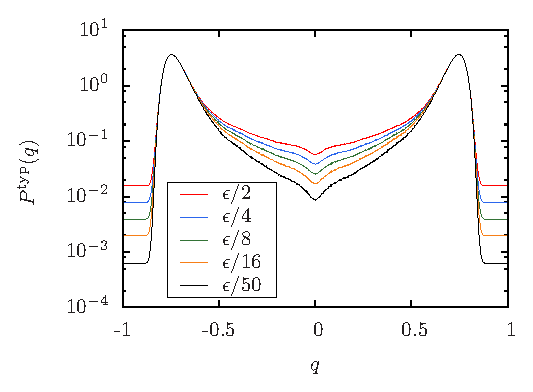
\includegraphics{import/EP}
  \caption
  [
    ``Typical" overlap distribution for the Sherrington-Kirkpatrick spin glass
    for various zero-replacement values $\epsilon/k$.
  ]
  {
    Log-linear plot of $P^{\mathrm{typ}}(q)$ for the SK model with $N=2048$,
    showing the strong dependence on the zero-replacement value $\epsilon/k$.
  }
  \label{fig:pofq-typical-sk}
\end{figure}


\section{Summary and conclusions}

We have studied the overlap distribution for several Ising spin-glass models
using recently-proposed observables. We consider 1D long-range models, 3D and
4D short-range (Edwards-Anderson) models, and the infinite-range
(Sherrington-Kirkpatrick) model. The three observables are all obtained from
the single-sample overlap distribution $\sample{P}(q)$. They are the fraction
of peaked samples $\Delta(q_0,\kappa)$, the median of the cumulative
distribution $I^{\mathrm{med}}(q)$, and the typical value of the distribution
$P^{\mathrm{typ}}(q)$. These observables were proposed to help distinguish
between the replica symmetry breaking picture and two-state pictures such as
the droplet model. While none of these unambiguously differentiates between
these competing pictures, it appears that $\Delta$ does the best job. In
particular, there is a qualitative distinction between the behavior for the 3D
EA model and the long-range 1D model with $\sigma=0.896$ that is expected to
mimic it, on the one hand, and the mean-field SK model and the 1D model with
$\sigma=0.6$ that is expected to be in the mean-field regime, on the other
hand. For a reasonable range of $q_0$ and $\kappa$, the two 3D-like models do
not show an increase in $\Delta$ for the largest sizes while the mean-field
models are sharply increasing for the largest sizes. The increase in $\Delta$
for the mean-field model is exactly what we expect from the RSB picture. The
results for the 3D-like models are ambiguous because eventually $\Delta$ must
go either to zero or one. It is possible that tfor much larger sizes $\Delta$
will begin to increase, indicating RSB behavior, but simulating such large systems
at very low temperatures is infeasible at present.

The other proposed measures do not appear to be useful in numerical simulations
for distinguishing scenarios. The typical value of the overlap distribution,
$P^{\mathrm{typ}}(q)$ cannot be measured in feasible Monte Carlo simulations,
while the median value of the cumulative overlap $I^{\mathrm{med}}(q)$ is very
small at small $q$ even for the SK model and has a very strong size dependence.
For the droplet model $I^{\mathrm{med}}(q)$ is presumably zero at small $q$ for
$N \to \infty$. However, the strong size dependence of the results in this
region of small $q$ makes it impossible to tell numerically if the data are
going to zero or just to a very small value, even for the SK model. Curiously,
there is \emph{less} size dependence for the 3D model and the equivalent 1D LR
model with $\sigma=0.896$ than for the SK model.

In contrast to the findings of \textcite{billoire2014cumulative} that the data
for $I^{\mathrm{med}}(q)$ for the SK model ``converge nicely to some limiting
curve when $N$ increases" and that ``trading the average for the median does
make the analysis more clear-cut," we find a strong size-dependence for
$I^{\mathrm{med}}(q)$ for te SK model in the important small-$q$ region
(clearly visible in a logarithmic scale) and largely because of this we do not
find that the median is particularly helpful in distinguishing between the
droplet and RSB pictures.
